
\title{The package Tikz-MultInets}

\author{Sallaccio}


\maketitle 

\begin{abstract}
We describe here the use of the package \thisPackage, an \emph{extended version} of a package written by Marc De Falco to represent interaction nets. 
His package was meant to represent simple interaction nets, i.e. with one principal port and simple wires as well as boxes and exponential boxes for linear logic. 
We added the possibility of defining cells with multiple principal ports, cells with only one port at all as well as many different ways of defining new paths for wires.
\end{abstract}




\section{Introduction}
The package uses mainly Tikz to create graphical representations of the most general case of interaction nets, i.e. interaction nets with multiport cells and multiwires.
Whereas the original package was aimed at the 

The package is meant to be retro-compatible with \inetPackageLong which was aimed at representing interaction nets as intended by Laffont.
All original commands are maintained and new commands were created in the same spirit,
thus the sporadic use of french names for some of the objects.


\section{Main extensions from original package}

Modifications from \inetPackageLong:
\begin{enumerate}[--]
\item apex angle of simple cells (from 60 to 100)
\item added multiport cells and 1-port cells
\item added multiwires
\item added empty node with anchors above and above above for better building of wires
\item added external auxiliary and principal ports to bypass cells
\item added commands for : cellheight, size of principal port in multicells, port size, free wire size, bypass distance
\end{enumerate}


\section{Macro usage}

\subsection{Global rules}

Some generic rules apply for all commands.


Arguments between square brackets -- /[/\metablue{options}/]/ -- are optional and may or may not have a default value.
They will be usually marked in blue.
For instance, \meta{direction} is always optional and has default value /D/, for \emph{down}.
This default value can be globally modified (see \ref{sec:packageSettings}).

The optional arguments in square brackets right after the command name are usually \meta{tikz-options} 
that change or overwrite graphical options for the given entity, cell or wire. 
See the Tikz package for more details.

Arguments between braces -- /{/\metared{options}/}/ -- are mandatory. 
In general, the red colour will be used to emphasize the fact that a value is {\color{red}\textbf{mandatory}}.

Sometimes, in some contexts, some arguments don't make much sense.
Then, an otherwise mandatory option can be skipped and the default value is used. 
In that case, it will be shown in orange -- /{/\metaorange{position}/}/.
This is mainly true of the position of a cell in the case it is the unique cell in the picture.
Its value is then equivalent to /{0,0}/\footnote{To say the truth, 
in such a case any position value would give the same result since images are cropped.}.
Note that if it is ommited, in order for the parser to understand the omission, the command needs to have an explicit [\metablue{direction}] or end with a semicolon \lq{\color{red};}\rq.

Finally, the elements' naming mechanism -- normal parenthesis, /(/\metaorange{name}/)/ -- follows Tikz' rules and is mandatory except if \meta{label} is simple, 
in which case the cell is implemented with the name \meta{label} 
(again, see Tikz package for details).


\subsection{Cells}

\subsubsection{The cell itself}

\DescribeMacro\inetmulticell
\optionskip/[/\metablue{options}/](/\metaorange{name}/){/\metared{label}/}{/\metared{coarity}/}{/\metared{arity}/}{/\metaorange{position}/}[/\metablue{direction}/]/

\metabold{options} can be a tikz-style, predefined style or any options for tikz lines.

\metabold{name} is a name to reference the object when building wires and ports. 

\metabold{label} is the label of the cell. It appears inside.

\metabold{coarity} is the number of \emph{principal ports} of the cell.

\metabold{arity} is the number of \emph{auxiliary ports} of the cell.

\metabold{position}  is a position in tikz-style cartesian or polar coordinates.

\metabold{direction} is either /D/ (default)/,L,U,R/ or any angle where `0' is down.

\medskip

\exampleNet{\inetmulticell(rho){$\rho_n$}{5}{3};}

\medskip
\noindent The length of a cell depends on the value of \meta{coarity}: it is defined as \meta{coarity}$\times$/\portsize/. 
If \meta{coarity}=1, then the constructed multicell will be an /\inetcell/ (see below).
If \meta{coarity}=1 and \meta{arity}=0, then the constructed multicell will be an /\inetzerocell/.
A special writing is allowed for cases where positionning is not done by coordinates (e.g. in /matrix/ environments). In such a case the \meta{position} can be ommited (equivalent to /{0,0}/ or /{0:0}/) but then the command should finish with a `;' or a \meta{direction}.

\medskip
\exampleNet{\inetmulticell(rho){$\rho_n$}{3}{3}{0,0}[65];}
\medskip
\exampleNet{\inetmulticell(rho){$\rho_n$}{3}{3}{0,0}[R];}
\bigskip
 
\DescribeMacro\inetcell
\optionskip/[/\metablue{options}/](/\metaorange{name}/){/\metared{label}/}{/\metaorange{position}/}[/\metablue{direction}/]/

\metabold{options} can be a tikz-style, predefined style or any options for tikz lines, 
or \texttt{arity=$k$} to create a cell with $k$ auxiliary ports.

\metabold{name} is a name to reference the object when building wires and ports. 

\metabold{label} is the label of the cell. It appears inside.

\metabold{position}  is a position in tikz-style cartesian or polar coordinates.

\metabold{direction} is either /D/ (default)/,L,U,R/ or any angle where `0' is down.

\medskip
\exampleNet{\inetcell(A){A}{0,0}[U];}
\bigskip

\DescribeMacro\inetzerocell
\optionskip/[/\metablue{options}/](/\metaorange{name}/){/\metared{label}/}{/\metaorange{position}/}/

\metabold{options} can be a tikz-style, predefined style or any options for tikz lines.

\metabold{name} is a name to reference the object when building wires and ports. 

\metabold{label} is the label of the cell. It appears inside.

\metabold{position}  is a position in tikz-style cartesian or polar coordinates.

\medskip
\exampleNet{\inetzerocell(Z){Z}{0,0};}


\subsubsection{Then its ports}


\DescribeMacro\inetport
\optionskip/[/\metablue{options}/](/\metared{port name}/)/

\metabold{options} can be a tikz-style, predefined style or any options for tikz lines.

\metabold{port name} is the complete name of a port.

\begin{exampleBox} 
\begin{verbatim}
\inetmulticell(rho){$\rho_n$}{5}{3};
\inetport(rho.pal 1)
\inetport(rho.pal 4)
\inetport(rho.pax 2)
\end{verbatim}		
\tcblower
\begin{center}
\begin{tikzpicture}
	\inetmulticell(rho){$\rho_n$}{5}{3};
	\inetport(rho.pal 1)
	\inetport(rho.pal 4)
	\inetport(rho.pax 2)
\end{tikzpicture}
\end{center}
\end{exampleBox}

\DescribeMacro\inetwirefree
\optionskip/[/\metablue{options}/](/\metared{port name}/)/

\metabold{options} can be a tikz-style, predefined style or any options for tikz lines.

\metabold{port name} is the complete name of a port.

\medskip
\DescribeMacro\inetbrace
\optionskip/(/\metared{first port}/)(/\metared{last port}/){/\metared{description}/}/

\metabold{first port} is the complete name of a port.

\metabold{last port} is the complete name of a port.

\metabold{description} is the text over the brace.

\subsection{Defining usefull cells}

This is a macro that enables to predefine a cell with particular label, coarity, arity and possibly direction.

\DescribeMacro\inetmulticelltype
\optionskip/[/\metablue{options}/]{/\metared{label}/}{/\metared{coarity}/}{/\metared{arity}/}/

\metabold{options} can be a tikz-style, predefined style or any options for tikz lines.

\metabold{label} is the label of the cell. It appears inside.

\metabold{coarity} is the number of \emph{principal ports} of the cell.

\metabold{arity} is the number of \emph{auxiliary ports} of the cell.

\metabold{direction} is either /D/ (default)/,L,U,R/ or any angle where `0' is down.

\noindent It is used inside a /\newcommand/ as follows:

\medskip
/\newcommand{\/\metared{specialcommand}/}{\inetmulticelltype/\ldots/}/
\medskip

\noindent It is then possible to define such a predefined cell by just giving its name and its position:

\medskip
/\/\metabold{specialcommand}/[/\metablue{new options}/](/\metared{name}/){/\metared{position}/}/
\medskip

Notice that \meta{new options} add up with options from the definition of the special command, and overwrite them in case of conflict.

For example:
%    \begin{macrocode}
		\newcommand{\alphacell}{\inetmulticelltype[very thick]{$\alpha$}{3}{2}}
		\alphacell[thin,minimum width=2ex](cellA){3,-1}
%    \end{macrocode}


\subsection{Wires}

The simplest wire is between two ports:
\medskip

\DescribeMacro\inetwire
\optionskip /[/\metablue{options}/](/\metared{port name}/)*</\metablue{cross node}/>(/\metared{port name}/)/

\metabold{options} can be a tikz-style, predefined style or any options for tikz lines.

\metabold{cross node} is optional nodes the wire should cross (see Section )

\metabold{port name} are complete names of ports. 

\medskip
Or between any two nodes:
\medskip

\DescribeMacro\inetwirecoords
\optionskip /[/\metablue{options}/](/\metared{node name}/)(/\metared{node name}/)/

\metabold{options} can be a tikz-style, predefined style or any options for tikz lines.

\metabold{node name} are any node name. 

\medskip
For some uses, when cells are really close, it might come in handy to use more flexible wires.
\medskip

\DescribeMacro\inetshortwire
\optionskip /[/\metablue{options}/](/\metared{port name}/)(/\metared{port name}/)/

\metabold{options} can be a tikz-style, predefined style or any options for tikz lines.

\metabold{port name} are complete names of ports. 

\medskip

\DescribeMacro\inetveryshortwire
\optionskip /[/\metablue{options}/](/\metared{port name}/)(/\metared{port name}/)/

\metabold{options} can be a tikz-style, predefined style or any options for tikz lines.

\metabold{port name} are complete names of ports. 

\medskip
Now the serious \emph{connectors}:
\medskip

\DescribeMacro\inetmultiwire
\optionskip/[/\metablue{options}/](/\metablue{name}/){/\metared{position}/}/

\hskip25pt/</\metablue{cross node}/>(/\metared{port 1}/)/

\hskip25pt/.../

\hskip25pt/</\metablue{cross node}/>(/\metared{port n}/)[/\mbox{\metablue{free port angle}}/]/

\metabold{options} can be a tikz-style, predefined style or any options for tikz lines.

\metabold{name} is a name for the wire. If not provided, no future use of it. 

\metabold{position} is a position in (cartesian or polar) coordinates for the wire.

\metabold{cross node} is optional nodes the wire should cross (see Section )

\metabold{port i} is a complete name of a port.

\metabold{free port angle} give the angle for the freeport if provided.

\medskip
At the center of a \emph{multiwire}, there is a visible /\inetnode/:
\medskip

\DescribeMacro\inetnode
\optionskip/[/\metablue{option}/](/\metared{name}/){/\metared{position}/}/

\metabold{option} can be `/wire/' or any options for tikz circle nodes.

\metabold{name} is a name for the wire. 

\metabold{position} is a position in (cartesian or polar) coordinates.

\medskip
\DescribeMacro\inetloop
\optionskip/[/\metablue{options}/]{/\metared{position}/}/

\metabold{options} can be a tikz-style, predefined style or any options for tikz lines.

\metabold{position} is a position for the center of the loop.

\medskip
\DescribeMacro\inetwirearoundleft
\optionskip/[/\metablue{options}/](/\metared{pal}/)(/\metared{pax}/)/

\metabold{options} can be a tikz-style, predefined style or any options for tikz lines.

\metabold{pal} is the complete name of a principal port of a cell.

\metabold{pax} is the complete name of an auxiliary port of a (usually the same) cell.

\DescribeMacro\inetwirearoundright
\optionskip/[/\metablue{options}/](/\metared{pal}/)(/\metared{pax}/)/

\metabold{options} can be a tikz-style, predefined style or any options for tikz lines.

\metabold{pal} is the complete name of a principal port of a cell.

\metabold{pax} is the complete name of an auxiliary port of a (usually the same) cell.

\medskip


\subsection{Boxes}

First a box around some nodes, then the promotion box of linear logic.
\medskip

\DescribeMacro\inetbox
\optionskip/[/\metablue{options}/]{/\metared{fit}/}(/\metared{name}/)/

\metabold{options} can be a tikz-style, predefined style or any options for tikz lines.

\metabold{fit} is a space-separated list of cell names /(a) (b) .../.

\metabold{name} is a name for further reference of the box. 

\DescribeMacro\inetprombox
\optionskip/[/\metablue{options}/]{/\metared{fit}/}(/\metared{name}/)/

\metabold{options} can be a tikz-style, predefined style or any options for tikz lines.

\metabold{fit} is a space-separated list of cell names /(a) (b) .../.

\metabold{name} is a name for the $!$-cell. The name of the box is /b/\meta{name}. 

\subsection{Relative positionning}

There are three main features of relative positionning.

\paragraph{Above a port}

\paragraph{Add a coordinate, cartesian or polar}

\paragraph{Crossings}


\section{Global values and defaults}

/\portsize/

\section{Here's the code}

\begin{macro}{slurp}

	\mbox{} blabla 
	
	dadf
	sdf
	sdf
%    \begin{macrocode}
      \begin{tikzpicture}
       bla
       
       blabla
      \end{tikzpicture}

%    \end{macrocode}

\end{macro}




\section{Creating wires}


%    \begin{macrocode}
	
	\begin{plouf}
	 Wasabi!
	\end{plouf}
	
%    \end{macrocode}




    
    
    
%    \begin{macrocode}
      
%    \end{macrocode}




\StopEventually{\PrintIndex}
\Finale

